\section{Implications for the study and optimization of \acs{WCA}}\label{sec:implications}
\todo[inline]{Implications for task durations, wrt to naive scheme.}
\todo[inline]{Implications for optimization in terms of sampling, energy.}
\todo[inline]{Introduction to this section}

\subsection{Application lifetimes}

We begin by studying the implications of such a model on the estimation of application lifetimes.
In the context of \ac{WCA}, we will understand \emph{application lifetime} as the time it takes a user to complete a specified task.
This is an important metric for \ac{WCA} optimization, as it directly relates to system resource utilization and contention, and to energy consumption.

In order to illustrate the consequences of using a less realistic model which does not take into account higher order effects, we introduce here a reference model to which we will compare our more realistic models.
This new model represents a first-order approximations the empirical execution time modeling, and consist simply of an \ac{exGaussian} distribution fitted to all execution time samples collected for \textcite{olguinmunoz:impact2021}.
This distribution is then randomly sampled at runtime to obtain execution times for each step, without any sort of adjustment to the current state of the system.

We start by studying application lifetimes in a controlled, ideal setup by using the timing models to generate execution times for sequences of \num{100} steps subject to constant \acp{TTF}.
These runs are completely simulated and no sampling of video frames is performed; for each step, we simply feed the models a predefined \acp{TTF} and record the generated execution time.
We use the combination of \acp{TTF} and execution times to calculate theoretical step duration times and subsequent total application lifetimes.
This is done for \num{25} linearly distributed \acp{TTF} in the \SIrange[]{0}{5}{\second} range; \num{45} independent repetitions for each combination of model configuration and \ac{TTF}.

\begin{figure}
    \centering
    \begin{subfigure}[]{\columnwidth}
        \centering
        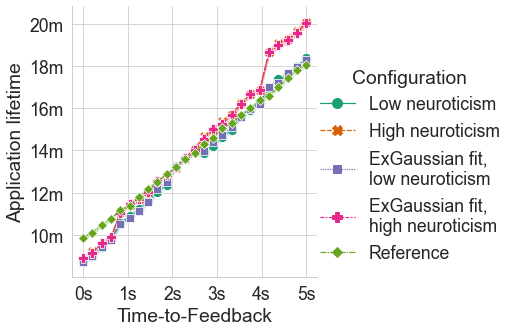
\includegraphics[width=.9\textwidth]{figs/new_model/lifetime_all_ttfs.png}
        \caption{%
            Evolution of application lifetimes as \acp{TTF} increase.
            Error bars indicate \SI{95}{\percent} \acp{CI}.
        }
    \end{subfigure}
    \begin{subfigure}[]{\columnwidth}
        \centering
        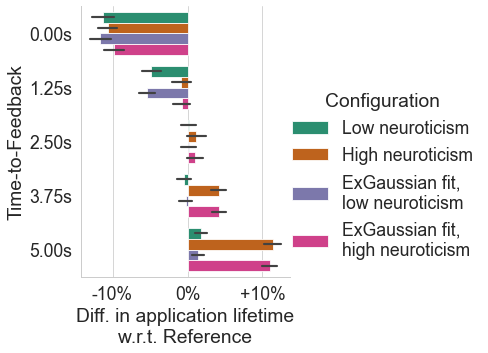
\includegraphics[width=.9\textwidth]{figs/new_model/lifetime_diff.png}
        \caption{%
            Percentage difference in mean application lifetimes with respect to the reference model at select \acp{TTF}.
            Error bars indicate the \SI{95}{\percent} \acp{CI}, calculated using a two-sided T-test.
        }
    \end{subfigure}
    \caption{\acl{TTF} versus application lifetime.}\label{fig:lifetimes}
\end{figure}

The results of this investigation are presented in \cref{fig:lifetimes}.
Compared to the reference model, our realistic models are, on average, roughly \SI{11}{\percent} faster when subject to low \acp{TTF}.
Conversely, at higher \acp{TTF} the relationship inverts, with the realistic models resulting in durations about \SI{2}{\minute} longer than the reference model, an increase of roughly \SI{11}{\percent}.

\todo[inline]{Discuss}

\begin{figure}
    \centering
    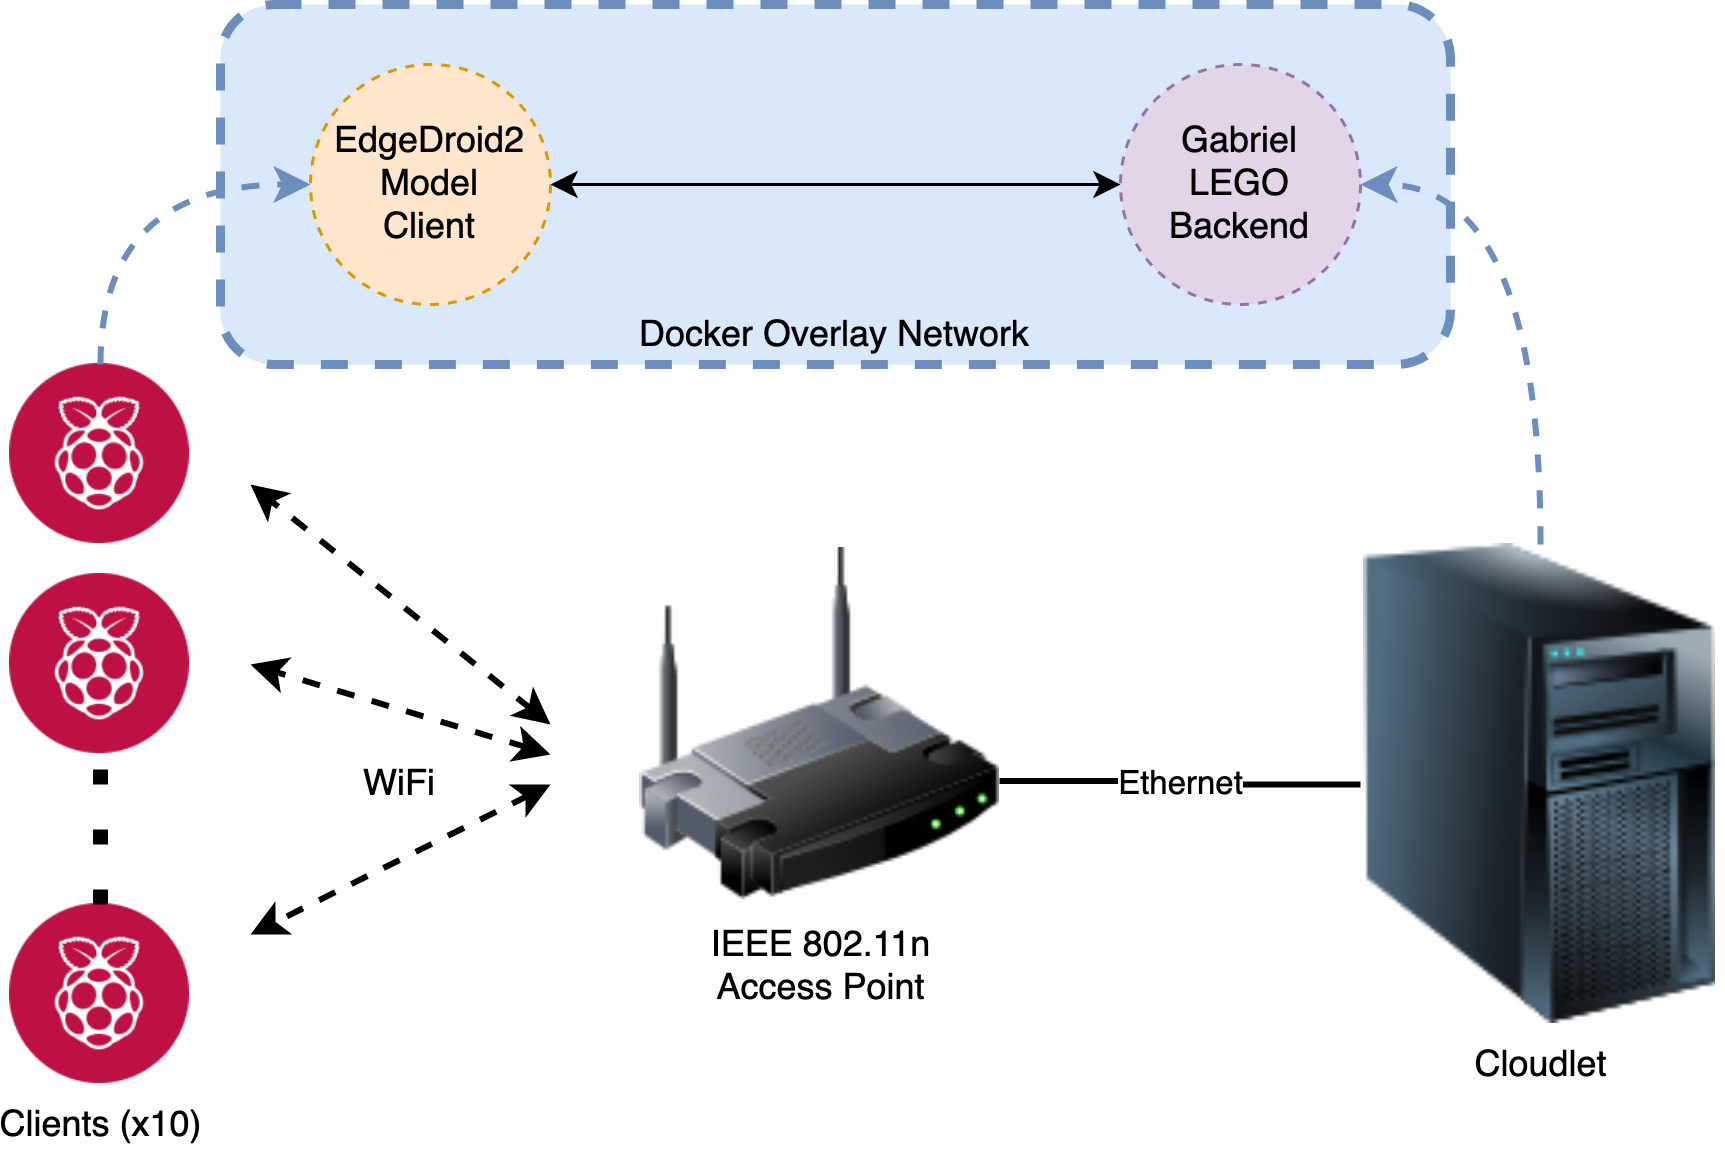
\includegraphics[width=\columnwidth]{figs/EdgeDroid2ExperimentalSetup.png}
    \caption{%
        Experimental setup used to study the implications of the realistic models of human behavior for \ac{WCA}.
        We deploy containerized instances of the client-server loop running the models on a testbed consisting of \num{10} Raspberry Pi clients connected to a cloudlet over a \ac{COTS} \acs{IEEE} \num{802.11}n access point.
    }\label{fig:expsetup}
\end{figure}

Next we study the effects of first- versus second-order models in a realistic setting.


\subsection{Energy consumption}

\todo[inline]{Add description of aperiodic sampling scheme}